%This is a comment

%each slide is defined with \begin{frame}{SLIDETITLE} ... \end{frame}
\begin{frame}{Contents}
\begin{enumerate}
  \item Motivation
  \item Greedy layer-wise unsupervised pretraining
  \item Transfer learning and domain adaptation
  \item Semi-supervised disentagling of causal factors
  \item Distributed representations
  \item Exponential gains from depth
  \item Ideas to discover underlying causes
\end{enumerate}
\end{frame}

%%this slide demonstrates how to include images 
%\begin{frame}{Figure}
%\begin{figure}[t]
%\centering
%\includegraphics[width=0.5\textwidth]{test_image.pdf} %the test_imgae is located in the "figures" folder. Place your figures there as well!
%\caption{Caption for the image}
%\end{figure}
%\end{frame}

\begin{frame}{Motivation}
The hardness of the task depends on how the information is presented:
\begin{itemize}
\item What is $\frac{CCX}{V}$?
\begin{itemize}
\item Ehm... What?
\end{itemize}
\item What is $\frac{210}{5}$?
\begin{itemize}
\item Easy! (42)
\end{itemize}
\end{itemize}

\end{frame}

\begin{frame}
What makes one representation of the information better than other?
\begin{itemize}
\item Inserting a number to a sorted list?
\begin{itemize}
\item $\mathcal{O}(n)$ if linked list
\item $\mathcal{O}(\log n)$ if red-black tree
\end{itemize}
\item Finding maximum from a sorted list?
\begin{itemize}
\item $\mathcal{O}(1)$ if linked list
\item $\mathcal{O}(\log n)$ if red-black tree
\end{itemize}
\end{itemize}
Subsequent tasks make the difference!
\end{frame}

\begin{frame}
How is this related to feed forward networks?
\begin{itemize}
\item E.G. for classification:
\begin{itemize}
\item Last layer performs linear classification
\item Rest of the layers provide a representation for this classifier
\end{itemize}
\item Every layer of a feed forward network can be thought as providing some representation of the data
\begin{itemize}
\item More interpretable near the end
\end{itemize}
\end{itemize}
\end{frame}

\begin{frame}
\begin{figure}[t]
\centering
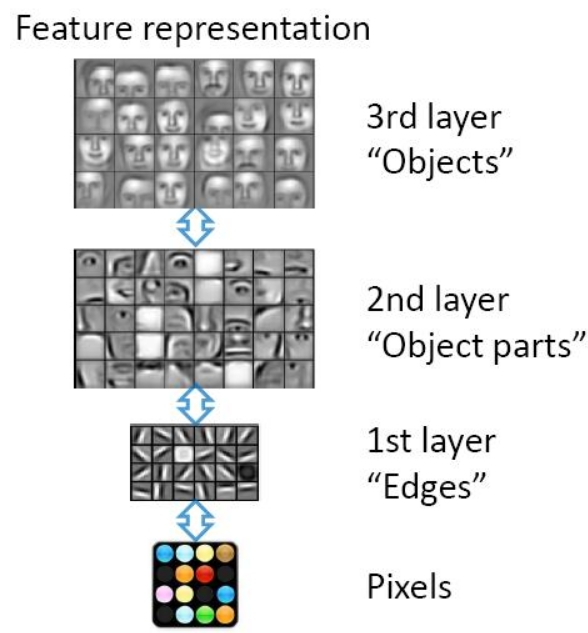
\includegraphics[width=0.50\textwidth]{features} %the test_imgae is located in the "figures" folder. Place your figures there as well!
\caption{Representations of different layers\footnote{\url{https://deeplearningworkshopnips2010.files.wordpress.com/2010/09/nips10-workshop-tutorial-final.pdf}}}
\end{figure}

\end{frame}

\begin{frame}
Consider following questions:
\begin{itemize}
\item What if we give the network some hints about good representations?
\item What if we reuse representation of some other network?
\item What if we use unlabelled data to find inlying structures?
\end{itemize}
Some answers to these questions provided in this presentation
\end{frame}

\begin{frame}{Greedy layer-wise unsupervised pretraining}
One way of unsupervised pre-training, dates back to 1975. General idea:
\begin{itemize}
\item Learn latent representation of a layer while keeping weights of previous layers fixed
\item Start from the first layer and proceed forward
\item Use some single layer representation algorithm such as Restricted Boltzmann Machines (RBM), auto-encoders or sparse coding models.
\item Fine-tune the networks with labelled data
\end{itemize}
\end{frame}

\begin{frame}
\begin{figure}[t]
\centering
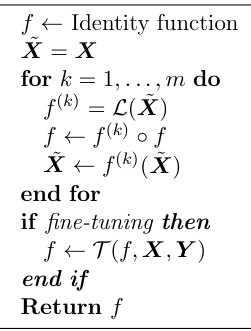
\includegraphics[width=0.40\textwidth]{alg15_1} %the test_imgae is located in the "figures" folder. Place your figures there as well!
\caption{Pseudo code for greedy layer-wise unsupervised pre-training. from Goodfellow \textit{et al.} (2016)}
\end{figure}
\end{frame}

\begin{frame}
Where does the algorithm name come from?
\begin{itemize}
\item{\bf greedy}: It optimises one part at a time
\item{\bf layer-wise}: optimises one layer at a time
\item{\bf unsupervised}: learning is done in an unsupervised manner
\item{\bf pretraining}: fine-tuning step is done after the pre-training part. 
\begin{itemize}
\item Can also be used as a pre-step for other unsupervised approaches 
\end{itemize}
\end{itemize}
\end{frame}

\begin{frame}
Why does the algorithm work?
\begin{itemize}
\item It regularizes
\begin{itemize}
\item Not well understood why
\item It is possible that pre-training initializes the weights to locations otherwise inaccessible (see Ehran et al (2010))
\begin{itemize}
\item Noisy gradients near the areas?
\item Badly conditioned Hessians?
\end{itemize}
\end{itemize}
\item Learning about the distribution can help in mapping 
\begin{itemize}
\item Not understood on mathematical level
\item Features that are found in unsupervised phase can be easily reused in classification
\end{itemize}
\end{itemize}
\end{frame}

\begin{frame}
When does the algorithm work?
\begin{itemize}
\item Big improvements in some problems, none in others. Might even decrease the performance in some cases.
\item Can be expected to be more effective if the initial representation is poor.
\begin{itemize}
\item Word representations are uninformative: Every two distinct one-hot vectors have same distance 
\end{itemize}
\item When number of labelled samples is small
\item When the number of unlabelled samples is large
\item If the learning task is complicated
\item If the network is deeper (see Ehran et al (2010))
\end{itemize}
\end{frame}


\begin{frame}
\begin{figure}[t]
\centering
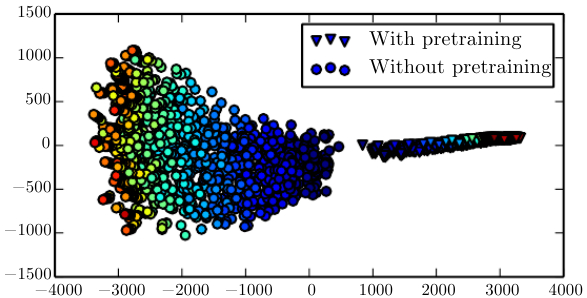
\includegraphics[width=1\textwidth]{pre_vs_no_pre} %the test_imgae is located in the "figures" folder. Place your figures there as well!
\caption{Visualization via nonlinear projection of the learning trajectories of different
neural networks in function space}
\end{figure}
\end{frame}


\begin{frame}
Discussion:
\begin{itemize}
\item Disadvantage in the method is that it has two phases:
\begin{itemize}
\item Many hyper-parameters
\item How to control the regularization?
\item Performance of latter cannot be predicted during the first
\item Changing hyper-parameters of first phase takes long
\begin{itemize}
\item Use validation error of second phase to propose hyper-parameters for the first (Larochelle \textit{et al.} (2009))
\end{itemize}
\end{itemize}
\item Today, unsupervised pretraining is mainly used only in the field of natural language processing
\item Bayesian methods outperform pretraining based methods if not much data
\begin{itemize}
\item However, important milestone
\item has been generalised to supervised pretraining
\end{itemize}
\end{itemize}
\end{frame}
